\documentclass{beamer}
\usetheme[hideothersubsections]{AUTheme}
\setbeamertemplate{caption}[numbered]
\setbeamertemplate{bibliography item}[text]%,
\setbeamertemplate{footline}[frame number]

\usepackage[scaled]{helvet}

\usepackage{url}

\usepackage{tikz,pgf}
\usetikzlibrary{arrows}

\usepackage{epstopdf}
\usepackage{siunitx}
\usepackage{amsmath}
\usepackage{graphicx,subfigure}
\usepackage[maxcitenames = 1, mincitenames=1,backend=bibtex]{biblatex}
\usepackage{multicol}
\usepackage{wrapfig}
% \usepackage{minipage}
% \usepackage{../sty/media9/media9}
% \usepackage[utf8]{inputenc}
\usepackage{hypcap}
\usepackage{graphicx}
% used for image citations
\usepackage[absolute,overlay]{textpos}

\hyphenation{op-tical net-works semi-conduc-tor}

\title[DRTK Driver Assistance]{An On-Line Visual Driver Aid for\\ Safe and Precise Convoy Following in\\ Visibility-Impaired Conditions}
\author[]{Robert Cofield, Scott Martin, David Bevly}
\date{September , 2013} 

\newcommand{\citeitem}[1]{
  \emph{\citeyear{#1}}--\Citeauthor*{#1}, \citetitle{#1}
}


\AtBeginSection[] {
  \begin{frame}<beamer>
    \frametitle{Section Outline}
    \tableofcontents[currentsection,hideallsubsections]
  \end{frame}
}

\bibliography{../bib/master.bib}

%%%%%%%%%%%%%%%%%%%%%%%%%%%%%%%%%%%%%%%%%%%%%%%%%%%%%%%%%%%%%%%%%%%%%%%%%%%%%%%%

\begin{document}

%% Title Slide %%
\frame{\titlepage}

%%%%%%%%%%%%%%%%
%% Motivation %%
%%%%%%%%%%%%%%%%

\section{Motivation}

  %% Military 
  \begin{frame}{Military Convoying}
    \begin{figure}
      \includegraphics[width=5cm]{../graphics/convoy_sandstorm_orange.jpg}
      \caption{\cite{convoy_dust_orange}}
    \end{figure}
  \end{frame} 

  %% ConOps
  \begin{frame}{Concept of Operation}

    \begin{figure}
      \includegraphics[width=0.8\textwidth]{../graphics/blackbox_flowchart.png}
    \end{figure}
    \begin{itemize}
      \item
      \item
      \item
    \end{itemize}
  \end{frame}


%%%%%%%%%%%%%%%%%%%%%%%%%%%%%%%%
%% Literature & Previous Work %%
%%%%%%%%%%%%%%%%%%%%%%%%%%%%%%%%

\section{Literature}

  \subsection{DRTK}

    %% brief explanation
    \begin{frame}{Dynamic Base Real-Time Kinematic GNSS}
      \begin{itemize}
        \item LAMBDA Integer-Fixing Method
      \end{itemize}
    \end{frame}

    %% discuss accuracy
    \begin{frame}{Errors in DRTK}
    \end{frame}

  \subsection{TDCP}

    %% brief explanation
    \begin{frame}{Time-Differenced Carrier Phase GNSS}
    \end{frame}

    %% discuss accuracy
    \begin{frame}{Errors in TDCP}
    \end{frame}

  \subsection{Virtual Path}

    %% discuss virtual leader & path summation
    \begin{frame}{Construction of Path}
      \begin{figure}
        \includegraphics[width=10cm]{../graphics/path_algorithm.png}
      \end{figure}
    \end{frame}

%%%%%%%%%%%%%%%%%%%%%%%%%%%%%%%%%%%%
%% Presentation of final products %%
%%%%%%%%%%%%%%%%%%%%%%%%%%%%%%%%%%%%

\section{GUI}


  % Transition slide from Literature
  % Talk about waypoint following with Prowler
  \begin{frame}{Real-Time Implementation}
    \begin{minipage}{0.45\textwidth}
      \centering
      \includegraphics[width=\textwidth]{../graphics/data_algo.png}
    \end{minipage}
    \begin{minipage}{0.45\textwidth}
      \begin{itemize}
        \item Unmanned Following
        \item Waypoint-based control
      \end{itemize}
    \end{minipage}
  \end{frame}


  \begin{frame}{Initial Design Goals}
    \begin{itemize}
      \item
    \end{itemize}
  \end{frame}


  \subsection{Qt}

    \begin{frame}{Qt-Based GUI --- Data Display}
      \begin{figure}[ht] \centering
        \includegraphics[width=4in] {../graphics/final_design_data.png}
        \caption{Qt GUI in normal operation} \label{fig:qt_data_display}
      \end{figure}
    \end{frame}

    \begin{frame}{Qt-Based GUI --- Controls}
      \begin{figure}[ht] \centering
        \includegraphics[width=4in] {../graphics/final_design_opts.png}
        \caption{Qt GUI displaying view control data} \label{fig:qt_controls}
      \end{figure}
    \end{frame}

  \subsection{Earth}

    \begin{frame}{Google Earth GUI --- Data Display}
    \end{frame}

    \begin{frame}{Google Earth GUI -- Controls}
      \begin{figure}
        \includegraphics[width=0.9\textwidth]{../graphics/earth_slow.png}
      \end{figure}
    \end{frame}

  \subsection{Middleware}

    % talk about MOOS , etc
    \begin{frame}{Middleware}
    \end{frame}

    %% introduce interpolation
    \begin{frame}{Interpolation}
      \begin{figure}[ht] \centering
        \includegraphics[width=5cm] {../graphics/middleware_diagram.png}
        \caption{Data input procedure} \label{fig:mw_diagram}
      \end{figure}
    \end{frame}


%%%%%%%%%%%%%%%%%%%%%%%%%%%%%%%%%%%
%% Tests that were run & Results %%
%%%%%%%%%%%%%%%%%%%%%%%%%%%%%%%%%%%
\section{Experimentation}

  \subsection{Hardware \& Setup}

    \begin{frame}{Hardware}

        \begin{minipage}{0.45\textwidth}
          \centering
          \includegraphics[width=4cm]{../graphics/hardware_flow.png}
        \end{minipage}
        \begin{minipage}{0.45\textwidth}
          \begin{itemize}
            \item Novatel Propak v3 (OEMV board) L1/L2
            \item Pinwheel Antenna
            \item Digi Extend 900 Mhz radio
          \end{itemize}
        \end{minipage}

        \begin{figure}
          \includegraphics[width=4cm]{../graphics/lead_hardware.jpg}
        \end{figure}

    \end{frame}


    \begin{frame}{Presentation to Driver}

      \begin{figure}[ht] \centering
        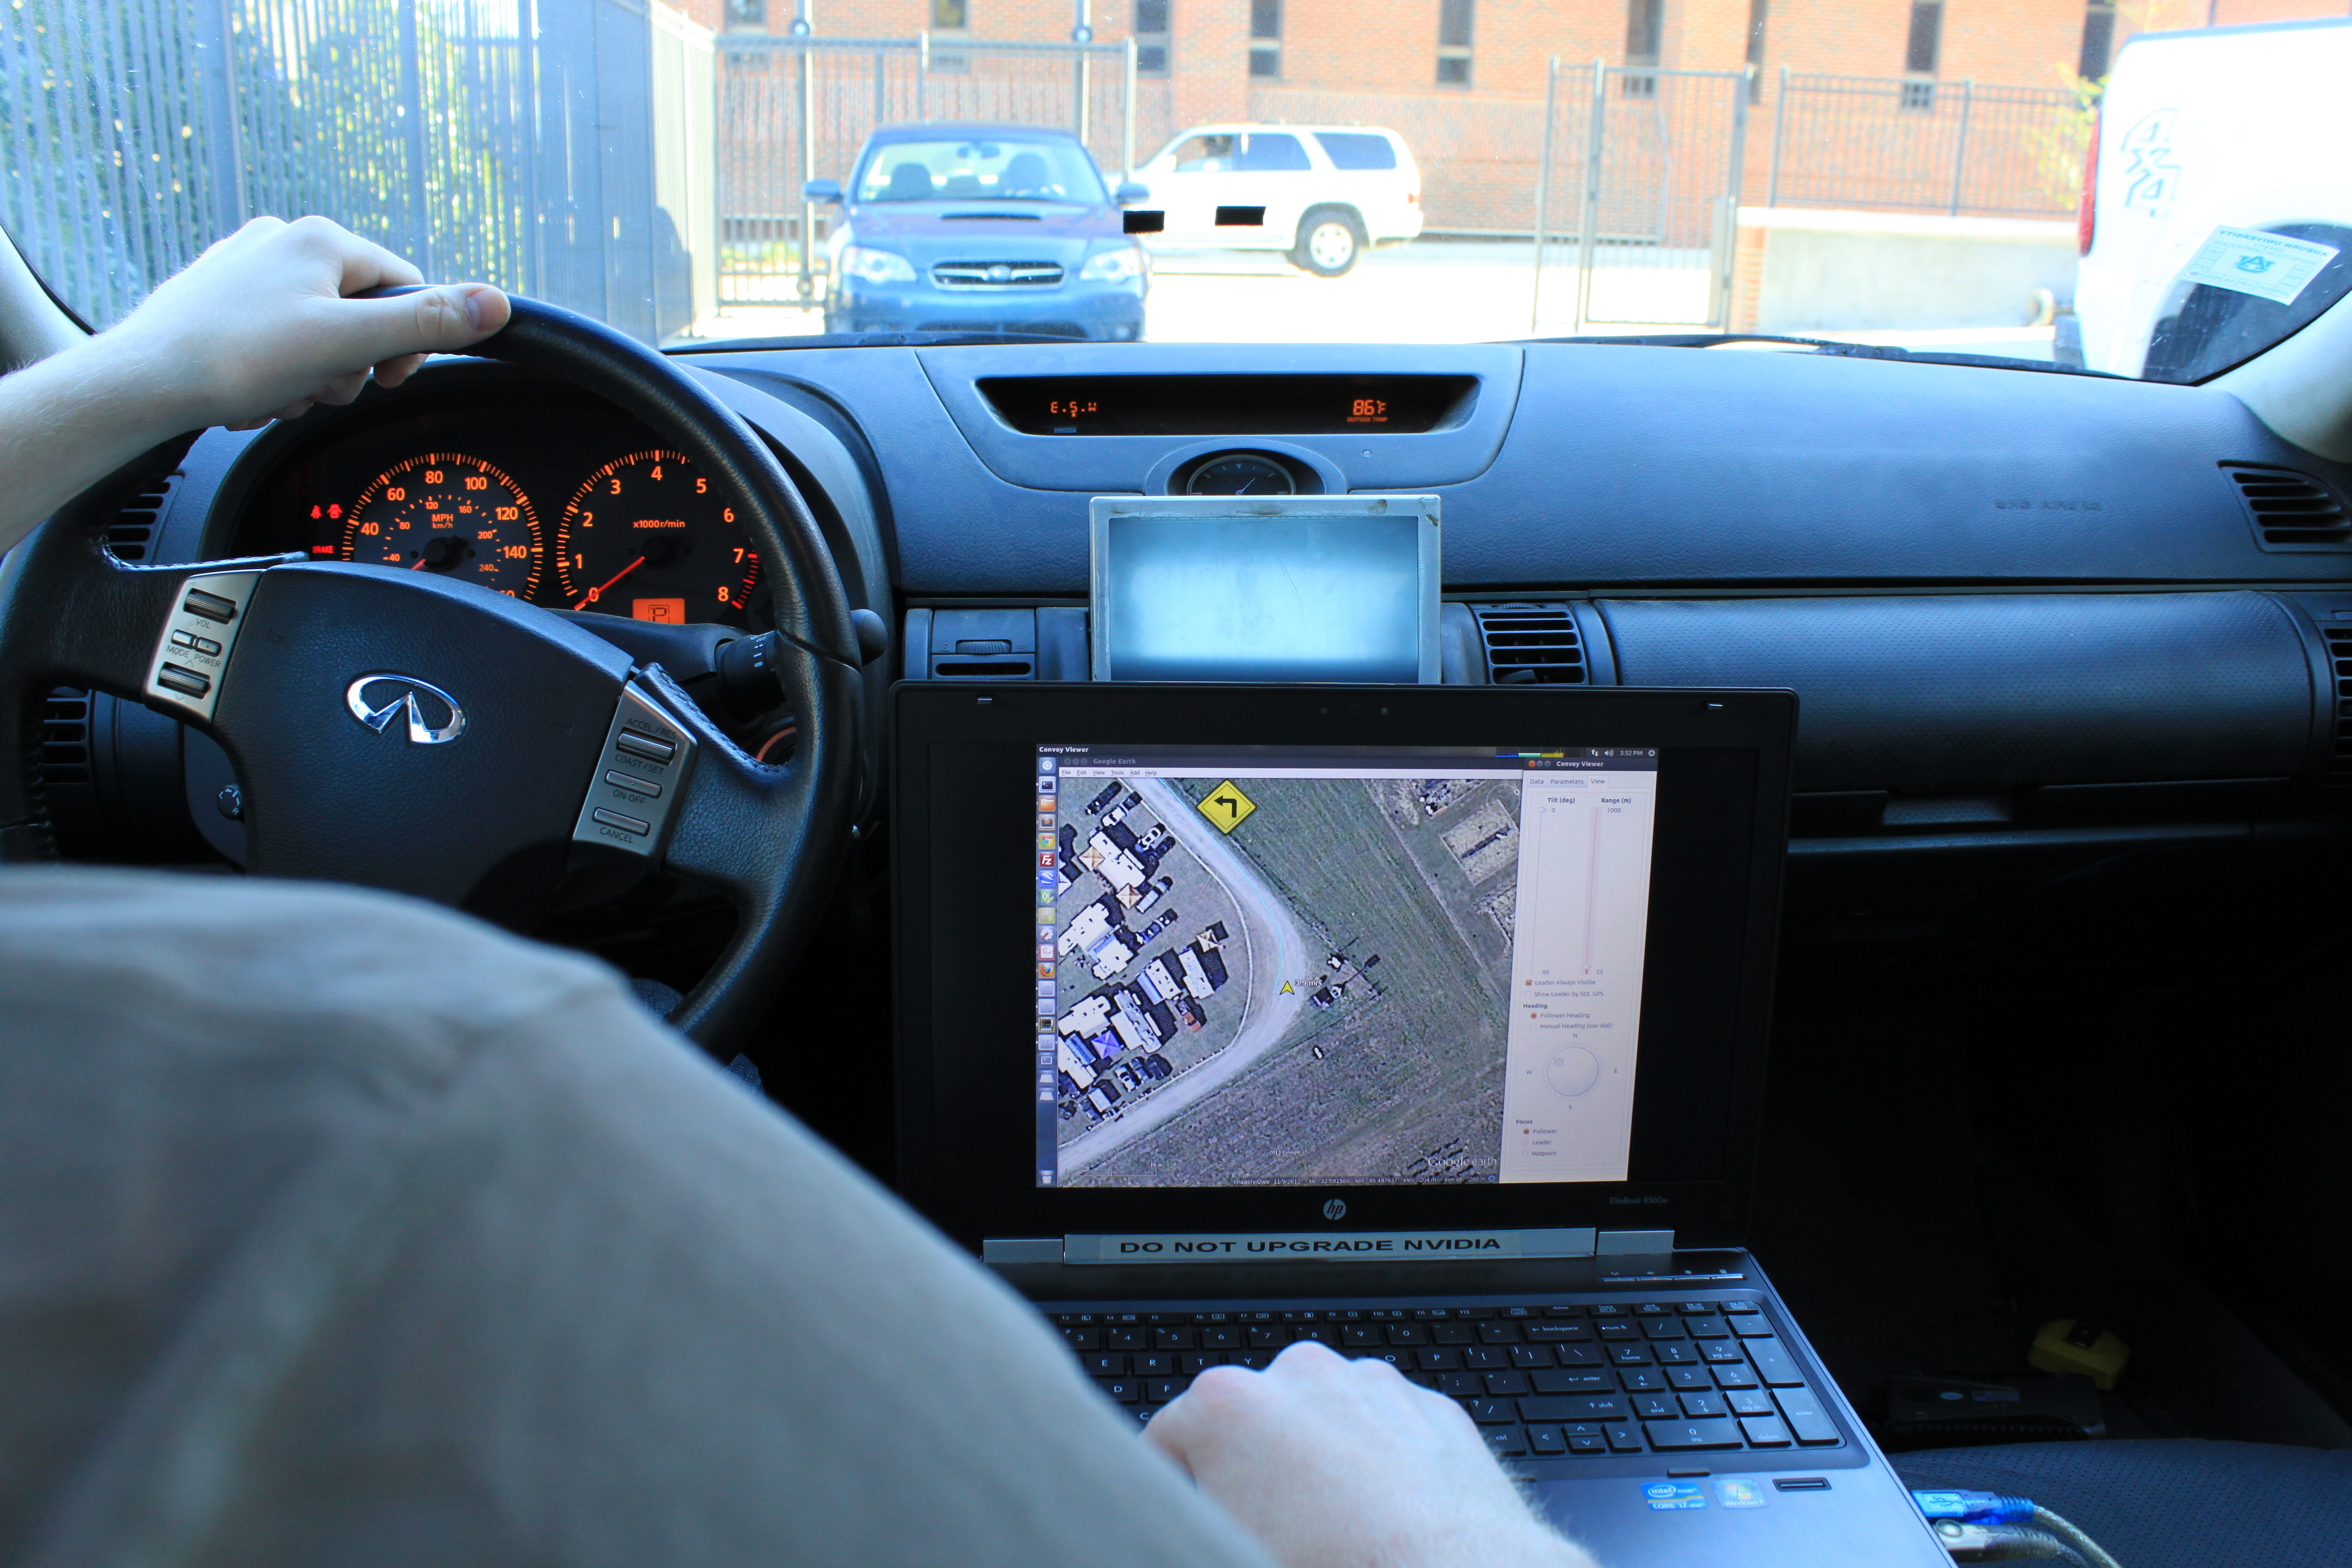
\includegraphics[width=5cm] {../graphics/driver_view.jpg}
        \caption{View from the driver's seat} \label{fig:driver_view}
      \end{figure}

    \end{frame}


  \subsection{Testing Procedures}

    % Outline of tests
    \begin{frame}{Testing Procedures}
    
      Lane Change Test

      Precision Following Test
      
      Zero Landmark Test

    \end{frame}

    \begin{frame}{Lane Change Test}
      \begin{figure}
        \input{../graphics/lane_change_diagram}
      \end{figure}
      % text describing test
    \end{frame}

    \begin{frame}{Precision Following Test}
      \begin{figure}
        \includegraphics[width=10cm]{../graphics/precision_following_diagram.png}
      \end{figure}   
    \end{frame}

    \begin{frame}{Zero Landmark Test}
      \begin{figure}
        \includegraphics[width=7cm]{../graphics/zero_landmark_path.png}
      \end{figure}
    \end{frame}


  \subsection{Results}

  %%% Lane Change Test
    % What the drivers saw in each GUI during the lane change
    \begin{frame}{Driver View}
      \begin{figure}[ht] \centering
        \begin{minipage}[b]{0.45\linewidth} \centering 
          \includegraphics[width=\textwidth]{../graphics/lane_change.png}
          \caption{Google Earth GUI approaching the lane change maneuver}
        \end{minipage}
        \hspace{0.5cm}
        \begin{minipage}[b]{0.45\linewidth} \centering
          \includegraphics[width=\textwidth]{../graphics/lane_change_mono.png} 
          \caption{Qt GUI approaching the lane change maneuver}
        \end{minipage}
    \end{figure}
    \end{frame}

    % present data
    \begin{frame}{Lane Change Test --- Results}
    \end{frame}

    % what happened
    \begin{frame}{Lane Change Test --- Discussion}
    \end{frame}

  %%% Precision Following Test
    % present data
    \begin{frame}{Precision Following Test --- Results}
      \begin{figure}
        \includegraphics[width=0.5\textwidth]{../graphics/precision_following_alert_percents.png}
      \end{figure}
      \begin{figure}
        \includegraphics[width=0.5\textwidth]{../graphics/precision_following_mu_distribution.png}
      \end{figure}
    \end{frame}

    % present data
    \begin{frame}{Precision Following Test --- Discussion}
    \end{frame}

  %%% Zero Landmark Test
    % present data
    \begin{frame}{Zero Landmark Test ---  Results}
    \end{frame}

    % what happened
    \begin{frame}{Zero Landmark Test ---  Discussion}
    \end{frame}


%%%%%%%%%%%%%%%%
%% Conclusion %%
%$%%%%%%%%%%%%%%
\section{Conclusion}

  \begin{frame}
  \end{frame}

\end{document}